\documentclass[a4paper,12pt]{report}

\usepackage{geometry}
\geometry{
    a4paper,
    lmargin=25mm,
    tmargin=25mm,
    rmargin=25mm,
    bmargin=25mm,
}

\usepackage{float}
\usepackage{cleveref}

\usepackage[american]{babel}
\usepackage{csquotes}

\usepackage{graphicx}
\graphicspath{ {images/} }

\usepackage{csquotes}
\usepackage[style=apa]{biblatex}
\newcommand{\citet}[1]{\citeauthor{#1} \shortcite{#1}}
\newcommand{\citep}{\cite}
\newcommand{\citealp}[1]{\citeauthor{#1} \citeyear{#1}}
\addbibresource{references.bib}

\usepackage{setspace}
\setstretch{2}

\usepackage[explicit]{titlesec}

\titleformat{\section}
  {\normalfont}{\thesection}{1em}{\centering{\textbf{#1}}{\setstretch{0}}}

\titleformat{\subsection}
  {\normalfont}{\thesection}{1em}{\textbf{#1}}{\setstretch{0}}

\titlespacing{\section}{0pt}{\parskip}{-\parskip}
\titlespacing{\subsection}{0pt}{\parskip}{-\parskip}

\usepackage{ragged2e}
\setlength{\RaggedRightParindent}{1.25cm}


\makeatletter
\renewcommand\tableofcontents{%
    \section*{\contentsname
        \@mkboth{%
           \MakeUppercase\contentsname}{\MakeUppercase\contentsname}}%
    \@starttoc{toc}%
}
\makeatother

\AddToHook{cmd/section/before}{\clearpage}

\tolerance=1
\emergencystretch=\maxdimen
\hyphenpenalty=10000
\hbadness=10000

\usepackage{enumitem}
\setlist{nosep}

\usepackage{multirow,booktabs,setspace,caption}
\usepackage{tikz}
\captionsetup[figure]{labelsep=period,labelfont=it,justification=justified,
  singlelinecheck=false,font=doublespacing}

\begin{document}

\RaggedRight

\begin{titlepage}
    \begin{center}
        \vspace*{1cm}
 
        \uppercase{National Research University Higher School of Economics}

        Saint Petersburg School of Economics and Management

        Department of Logistics and Supply Chain Management
         
        \vspace*{\fill}
            \textbf{\uppercase{Project Proposal:}}

            Automated Benchmarking of CVRP Solvers
        \vspace*{\fill}
 
        % \vfill
        
        \vspace*{\fill}
            \hspace*{0pt}\hfill Andrei A. Prokhorov

            \hspace*{0pt}\hfill BLG-203
            
            ~\\
            
            \hspace*{0pt}\hfill Academic Supervisor

            \hspace*{0pt}\hfill Nikolay N. Nikolayevskiy, Senior Lecturer

            ~\\

            \hspace*{0pt}\hfill Language Supervisor

            \hspace*{0pt}\hfill Vera M. Kartashova, Visiting Lecturer

        \vspace*{\fill}

        \centering{Saint Petersburg}

        \centering{\the\year{}}

    \end{center}
\end{titlepage}
\addtocounter{page}{1}

\setcounter{secnumdepth}{0}
\renewcommand{\contentsname}{\centering \normalsize \textbf Table of contents}
\newpage
  \tableofcontents
\newpage

\section{Abstract}

Modern logistics relies heavily on the vehicle routing problem (VRP), which offers an organized framework for assessing and applying algorithms to handle new distribution complexity, particularly regarding last-mile delivery. Nonetheless, the emerging complexity of solutions available today has raised concerns about the accessibility of contemporary evaluation, calling for the use of standardized and repeatable comparison techniques. As a result of the current state of benchmarking practice's lack of consistency and overlooking of best practice, such as algorithm parameters, there arise inconsistencies in evaluation results. This work aims to give a thorough review of current benchmarking best practice and propose a standardized way for assessing CVRP solvers. By delineating best practices and developing an experimental framework, this study aims to implement theoretical advancements into a practical implementation of CVRP solver comparison, establishing a robust basis for future benchmarking and ensuring transparency and rigor in the assessment of CVRP solvers.

\section{Introduction}

The vehicle routing problem is integral for modern logistics, as it provides a robust framework for assessing and applying algorithms to solve a number of distribution problems in logistic, commonly found among recently emerged last-mile delivery focused business models. This has attracted numerous researchers over several decades to introduce their own visions of the problem variant statements and solutions for them into the scientific community. The abundance of solutions to the problem may have threatened approachability of state-of-the-art assessment in this field, as it currently lacks proven to be reproducible comparison methods.

Multiple variants of the Vehicle Routing Problem have emerged so far. They vary in generality and constraint choices, but most common variants include parts of the following problem statements:

\begin{enumerate}
    \item VRPTW: Vehicle Routing Problem with Time Windows, in which periods of time the client can be reached in are specified as an additional constraint.
    \item MDVRP: Multi-Depot Vehicle Routing Problem, which states a more general variant of the vehicle routing problem, where there are multiple points where the fleet of vehicles has to start and finish their routes at.
    \item Stochastic VRP, that uses non-deterministic demand functions.
\end{enumerate}

Each of these and many other problem statements requires specific approaches in order to determine the optimal solution, but this paper is focused on CVRP as the subject, as the capacity constraint is included more frequently compared to any other constraint and is believed to be representative of a heuristic's applicability in other VRP variants.

Capacitated vehicle routing problem (CVRP), illustrated by figure \ref{fig:img_cvrp_example} is a vehicle routing problem in which a fleet of vehicles limited in capacity must deliver goods from one point to several destinations. Each destination has its own cargo demand, and the goal of the problem is to find a set of sub-routes for the vehicles starting and ending at the origin such that all destinations are visited, the sum of the demands on each sub-route does not exceed the vehicle's capacity, with the total distance traveled being minimized.

\begin{figure}[H]
    \centering
    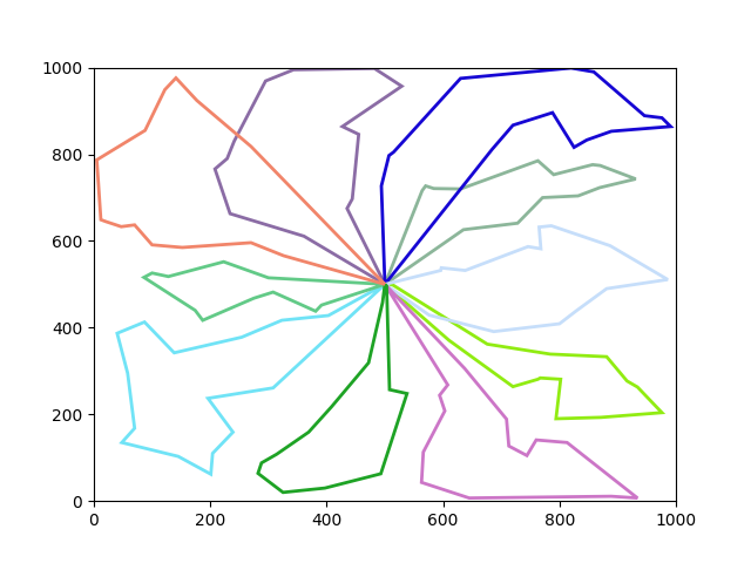
\includegraphics[
        width=0.6\textwidth
    ]{images/cvrp_example.png}
    \caption{
        A solution of the X bencharking set
        \autocite{uchoaNew}
        by the HGS algorithm
        \autocite{vidalHybridGeneticSearch2022}.}
    \label{fig:img_cvrp_example}
\end{figure}

CVRP is an NP-hard problem, thus most researchers focus on finding approximate methods of solving it. As illustrated in {figure \ref{fig:cvrp_solution_methods}, approximate solution methods are commonly separated into heuristics, which are specific to this particular problem, and metaheuristics, which are commonly applicable to a vast number of optimization problems.

\begin{figure}[H]
    \centering
    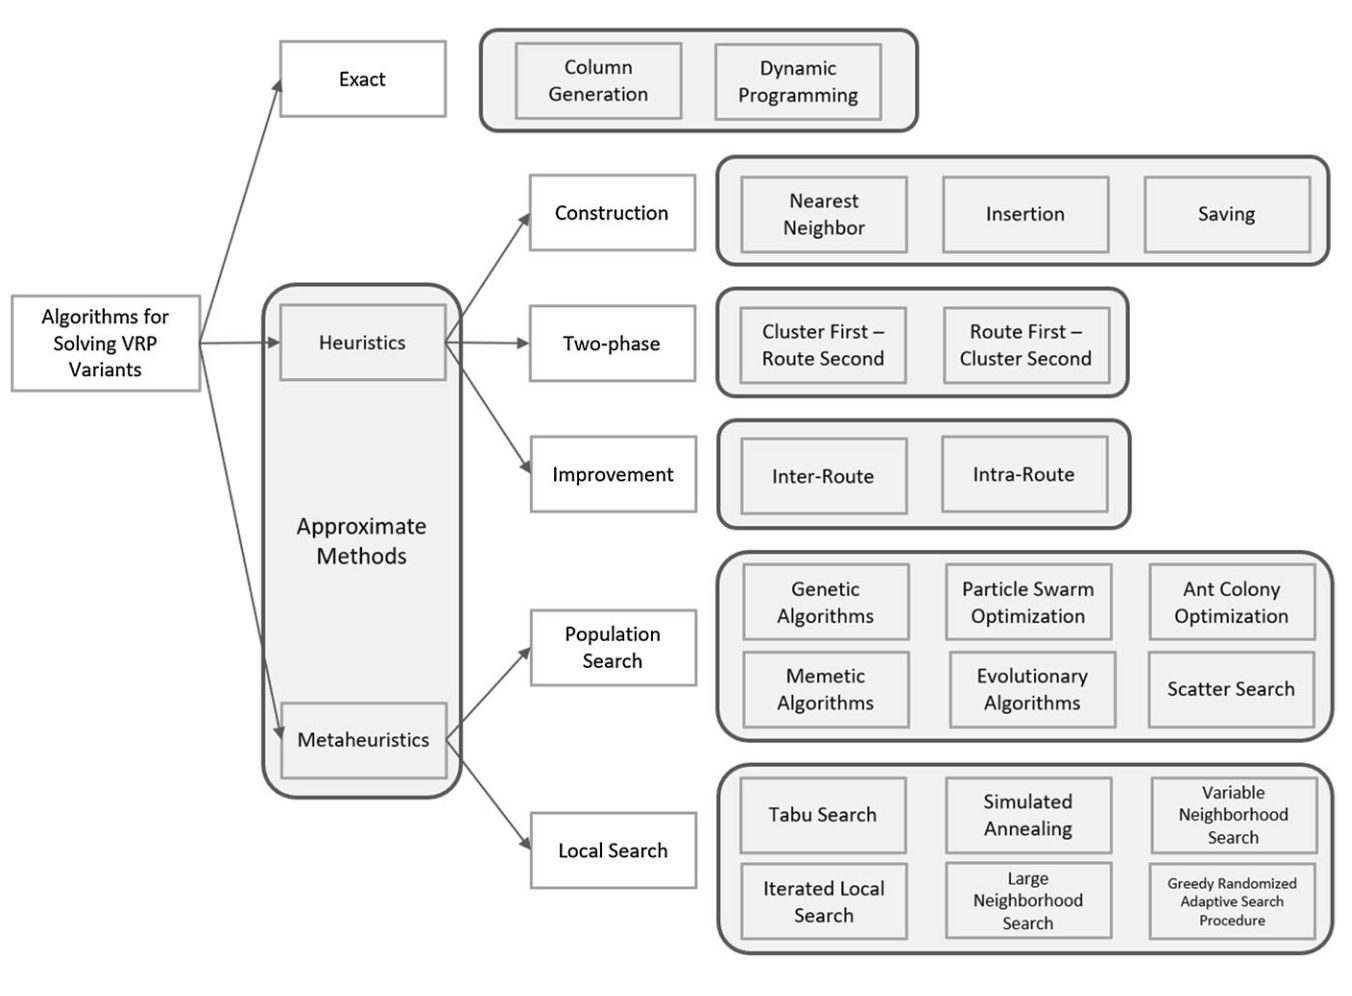
\includegraphics[
        width=0.6\textwidth
    ]{images/cvrp_solution_methods.png}
    \caption{
        Solution methods classified by \Citeauthor{konstantakopoulosVehicle} (\citeyear{konstantakopoulosVehicle}).}
    \label{fig:cvrp_solution_methods} 
\end{figure}

Many of current researchers when proposing their solvers tend to introduce their own comparison methodologies. When assessing the state-of-the-art in solvers for the Vehicle Routing Problem, it may introduce mutual inapplicability of comparisons from different papers, therefore creating a need for a further exhaustive comparison to address this.

This paper will attempt to introduce a comparison methodology based on benchmarking, asses its dependency of computational resources and several parameters on it to assess its environmental independency. A tool will be created, which may be used by CVRP researchers to compare their solvers.

\section{Literature Review}

\subsection{Current State of Comparison Methods}

Proposing a new heuristic to solve a vehicle routing problem, researchers include comparisons of their algorithm to ones arbitrarily chosen for that purpose. Typically, the algorithms are run on a single CPU core until a stop-conditon is reached. Parameters, which determine a proposed heuristic's behavior, are configured beforehand. A comparison is run on one or more benchmarking problem sets, developed separately from the solver. There is not much concern for memory used, as in the case of Vehicle Routing Problem computational complexity grows much faster, and memory usage is not monitored in the comparisons. CPU time and solution quality are examined with a greater dedication. 

Two indicative papers are presented to represent current state of benchmarking for CVRP solvers. Both papers present their proposed solvers as better than ones they have been compared to.

\Citeauthor{vidalHybridGeneticSearch2022} (\citeyear{vidalHybridGeneticSearch2022}) compares a proposed Hybrid genetic search-based solver to 8 other ones, which are described to represent the state-of-the-art: OR-Tools, HILS, LKH-3, KGLS, SISR, FILO, HGS-2012 and BKS. These solvers are run multiple times with chosen hyperparameters for said solvers not described. The authors use the X problem set for benchmarking. The set was introduced by \Citeauthor{uchoaNew} (\citeyear{uchoaNew}) with 100 instances and number of destination points ranging from 100 to 1000. The main metric is performance at target execution time, and at set fractions of it. The target execution time is linearly dependent on the number of destination points for each benchmark instance. While this comparison is relatively more comprehensive, it seems to fail to account for the impact of heuristic's parameters on its performance. For instance, having hyperparameters be independent of target time may result in a heuristic's inability to reach peak performance for set time. This may happen when the performance is a function of the number of iterations, such as in Simulated Annealing, a commonly used metaheuristic. It defines a probability of choosing a worse result during an iteration in permutation-based iterative heuristic algorithms as a linear or exponential function of current iteration number. The linear or exponential coefficients are set based on the overall number of iterations, irrelative of the target time, such that the probability reaches zero on the final iteration. This may impact the performance of a solver that implements such heuristic, if the target number of iterations is much greater than reasonable for chosen target time on a chosen machine. Moreover, there are no descriptions provided for the choice of comparison targets, target time and its fractions, and the number of times solvers are run with different seed values.

\Citeauthor{ahmedBilayer} (\citeyear{ahmedBilayer}) compare their proposed Particle Swarm based method with 4 other PSO-based solvers: DPSO, SR1, SR2 and PSCO. They use 6 benchmarking sets: A, B, E, F, M, P and CMT. These overall set consists of 106 problems ranging in number of destination points from 15 to 199. No description of hyperparameters used for said solvers is provided. The target metrics are best-found solution, average and best computational time for the number of iterations. The number of iterations is set to 50 for BLS-PSO, but it is unclear whether it is the case for other algorithms. The researchers state that the proposed algorithm is better than the chosen ones. The chosen benchmark instances are significantly smaller than those in the X set and the choice of target metrics is not substantiated. This choice of instances and solvers for comparison is not indicative of the state-of-the-art, as more complex instances have been introduced as of the publishing of that paper.

\subsection{Best Practice Overview}

In order to account for aforementioned potential problems in benchmarking of CVRP solvers, it is important to consider best practices.

\Citeauthor{beiranvandBest} (\citeyear{beiranvandBest}) describe a theoretical framework for benchmarking optimization methods, which include best practices in the following steps: clarifying the reasons for benchmarking, selecting the test set and performing the experiments.

In terms of reasoning for a benchmark, \Citeauthor{beiranvandBest} (\citeyear{beiranvandBest}) state, that it is a must to find the most important aspect of the algorithm and base the comparison on it. In the case of the Vehicle routing Problem, both time and precision matter, thus it is up to the user to determine which one is the primary concern. Regarding the comparison of VRP solvers, to provide better grounds for such a choice, there may be a need for a combined metric of time and precision.

Considering test sets, \Citeauthor{beiranvandBest} (\citeyear{beiranvandBest}) instruct to adjust the benchmarking set for the following considerations, applicable to CVRP benchmarking:

\begin{enumerate}
    \item One must avoid small problem sets for reliable conclusions;
    \item The tests should contain problems of varying difficulty, at least \emph{easy}, ie. solvable by most algorithms on a personal computer, and \emph{hard};
    \item There have to exist known solutions to at least a part of the problem set.
    \item One must examine the test set for possible patterns, that may provide advantage to some solvers.
\end{enumerate}

Test set X, introduced by \Citeauthor{uchoaNew} (\citeyear{uchoaNew}), addresses these concerns by making the set relatively vast, consisting of 100 problems, which is bigger than an arbitrary mark of 20, set by \Citeauthor{beiranvandBest} (\citeyear{beiranvandBest}). It does provide easy, medium and hard-difficulty problems, as separated by \Citeauthor{christiaensSlackInductionString2020} (\citeyear{christiaensSlackInductionString2020}) while comparing their solver with others. Smaller problems of the set have proven-minimum solutions and, finally, some parts of this set do include intentionally made patterns to account for real-world specifics, such as demand-distribution functions and clustered customer points.

When choosing a metric for the experiments, \Citeauthor{beiranvandBest} (\citeyear{beiranvandBest}) suggest to determine a resulting function, which, in case of CVRP is average difference from the best known solution. Additionally, they instruct to account for algorithm parameter's influence by means of their automatic tuning as a pre-processing step, which is not done in current practice.

Although current state of benchmarking lacks standardization of practice and consideration for algorithm parameters, it may be achieved. This paper's aim is thus to provide an example and create a practical framework for similar endeavors.

\section{Methodology}

To account for the lack of parameter tuning, Optuna library, proposed by \Citeauthor{akibaOptuna} (\citeyear{akibaOptuna}), will be used, as it is one of the most popular frameworks for hyperparameter tuning. The target function for both parameter tuning and running the experiments will be performance at set time. Number of iterations in solvers, which are dependent on it, will be interpreted as one of the parameters.
The X benchmarking problem set will be used as it provides variety in problem statements and complexity.
Several comparison parameters value's impact on comparison results will be evaluated. These parameters are: target time function formula and coefficient, number of iterations for hyperparameter tuning and number of iterations in experimental runs and heuristic used for hyperparameter tuning.
To assess how these parameters influence the benchmarking, the following steps will be done for several combinations of these values:

\begin{enumerate}
    \item Hyperparameter tuning. Hyperparameters are set to optimal values for a particular environment;
    \item Consecutive runs. Each algorithm, with its hyperparameters adjusted, is then run a set amount of times with different seed values to take randomness into consideration;
    \item Result distribution assessment. As the result distribution is unknown and may not be normal, a non-parametric Kolmogorov-Smirnov test was chosen to be the metric of sample difference for different algorithms' results.
\end{enumerate}

To assess the impact of the presence of hyperparameter benchmarking on the comparison result, runs with zero iterations for hyperparameter tuning will be executed.

\section{Anticipated Results}

The series of experiments will provide a mapping from target time function, the number of tuning and experiment runs and hyperparameter tuning function to solvers' run results. It will be possible to examine the possibility of determining the best configuration of these parameters for accurate and truthful benchmarking of CVRP solvers.
Several hypotheses will be tested: 

\begin{enumerate}
    \item Time function has influence on experiment results where the number of parameter tuning runs is lower.
    \item With growing number of experimental runs average run results will converge.
    \item Parameter tuning functions affect the experiment results.
\end{enumerate}

An automated tool for conducting similar experiments on various scales will be developed as a python library, available for free use.

\section{Conclusion}

With new CVRP solvers being introduced, more rigorous requirements for benchmarking tools are needed to preserve comprehensibility of state-of-the-art in this field.

While best practices include hyperparameter tuning, the current practice in CVRP benchmarking tends to overlook this matter, while also lacking standardization and reasoning behind chosen methods for benchmarking. This may lead to increased ambiguity and thus research costs for companies attempting to find heuristics to base their solvers on.

To address it, this study will attempt to compile known best practices for comparing heuristics into a cohesive benchmarking framework able to be used for CVRP solvers and explore some of its parameters impact on the quality of benchmarking. This will address an existing issue of lack of consideration for hyperparameter optimization in current CVRP solver benchmarking practice.

For researchers, such tool, if used widely, will decrease research time and increase comparability of their proposed solvers.

\printbibliography[heading=subbibintoc, title={\normalfont References}]

\end{document}
